%\begin{fullpage}

\section{Seminar - Anforderungsanalyse}

    \subsection{Aufgabe 1 - Pflichtenheft}
    
        \begin{aufgabe}
            Die Anforderungsanalyse ist ein wichtiger Teilschritt zu Beginn eines Softwareentwicklungsprozesses und ist der erste Schritt nach Erhalt des Lastenheftes Ihres Auftraggebers. Das Ergebnis der Anforderungsanalyse ist das Pflichtenheft als ein zentraler Ausgangspunkt des Entwicklungsprozesses. Welche Bestandteile und Informationen muss ein Pflichtenheft enthalten?
        \end{aufgabe}
        
        \begin{loesung}\:
            Ein Pflichtenheft beinhaltet die exakte Umsetzungsbeschreibung (Konkretisierung), der im Lastenheft formulierten Anforderungen und bildet die Grundlage für die vertraglich festgehaltenen Leistungen des Auftragnehmers. Genauer besteht ein Pflichtenheft grundsätzlich aus vier Teilen:
            \\[-.7cm]\begin{enumerate}
                \setlength\itemsep{0.1px}
                \item Genaue Beschreibung der gestellten Anforderungen
                \item Projektteilnehmer und Aufgabenverteilung
                \item Erfüllte Voraussetzungen
                \item Zeitlicher Rahmen des Projektes (wie und bis wann)
            \end{enumerate}
            Dabei sollten folgende Informationen bzw. Themen unbedingt im Pflichtenheft enthalten sein:
            \\[-.7cm]\begin{itemize}
                \setlength\itemsep{0.1px}
                \item Einführung - Informationen Auftraggeber/Auftragnehmer und Ansprechpartner
                \item Anlass des Projektes
                \item Ausgangslage
                \item Eindeutige Beschreibung der Projektziele, Aufgabenstellung, Rahmenbedingungen
                \item Schnittstellenbeschreibung
                \item Beschreibung geforderter Funktionalität
                \item Leistungsbeschreibung - Anforderungen an Funktionen
                \item Phasenplan/Eckdaten und Projektplan
                \item Beurteilung Machbarkeit, organisatorischer / technischer Aufwand
                \item Projektorganisation - wer macht was und wann
                \item Externe Einflüsse
                \item Testbetrieb
                \item Ablaufkontrolle
                \item Abnahme
            \end{itemize}
        \end{loesung}


    \subsection{Aufgabe 2 - Anforderungsdefinition}
    
        \begin{aufgabe}
            Die Anforderungsdefinition ist ein Teil des Pflichtenheftes.
            \\[-.7cm]\begin{enumerate}[(a)]
                \setlength\itemsep{0.1px}
                \item Stellen Sie ausgehend von der Beschreibung aus dem Video die funktionalen sowie nichtfunktionalen Anforderungen an das zu entwickelnde Umweltplaketten-Spiel auf. Halten Sie die Beschreibung der Anforderungen in Ihrem Dokument fest (z.B. in Form einer Liste oder einer Tabelle). Zur Beschreibung einer Anforderung sollen mindestens die folgenden Eigenschaften gehören:
                \\[-.7cm]\begin{itemize}
                    \setlength\itemsep{0.1px}
                    \item eine eindeutige ID (z.B. F01, F02, ... für funktionale, NF01, NF02, ... für nichtfunktionale Anforderungen)
                    \item ein für den Menschen verständlicher Name
                    \item die eigentliche Beschreibung
                    \item Ihre Bewertung der Priorität der Anforderung (z.B. nach 'Muss', 'Kann/Sollte' und 'Optional/Nice-to-have') 
                \end{itemize}
                \item In der Vorlesung haben Sie etwas über Meta-Anforderungen, also Anforderungen an Anforderungen gelernt (z.B. Vollständigkeit, Eindeutigkeit, Korrektheit, usw.). Überprüfen Sie, ob die von Ihnen aufgestellten Anforderungen diesen Kriterien gerecht werden. Überarbeiten Sie Ihre Anforderungen gegebenenfalls. Am Ende sollen Ihre beschriebenen Anforderungen bestmöglich den Meta-Anforderungen genügen.
            \end{enumerate}
        \end{aufgabe}
    
        \begin{loesung}\:
            \\[-.7cm]\begin{enumerate}[(a)]
                \setlength\itemsep{0.1px}
                \item 
                    \textbf{Benutzerfunktionen}
                    \begin{description}
                        \item[/F0010-S/]
                        \textit{Registrieren:} Ein beliebiger Internet-Benutzer kann sich über die Start- bzw. Login- Seite des Systems schnell registrieren lassen. Zum Registrieren sind mindestens folgende Angaben erforderlich: gewünschter \textbf{Benutzername}, gewünschtes \textbf{Passwort}.
                        
                        Die Registrierung auf der Seite ist rein optional und dient lediglich der Speicherung des Highscores. Der Internet-Nutzer kann auch spielen, wenn er nicht registriert ist, wobei sein Punktestand jedoch nicht gespeichert werden kann.
                        
                        Mit dem erfolgreichen Abschießen des Registrierungsvorgangs ist der neue Benutzer am System angemeldet.
                        
                        \item[/F0020-S/]
                        \textit{Anmelden:} Ein bereits registrierter Benutzer kann sich über die Start- bzw. Login- Seite des Systems schnell und bequem anmelden (\textit{login}). Dazu ist seine Kennung (\textbf{Benutzername, Passwort}) erforderlich.
                        
                        \item[/F0030-S/]
                        \textit{Abmelden:} Der angemeldete Benutzer kann sich jeder Zeit wieder vom System \textbf{abmelden} (\textit{logout}).
                        
                        \item[/F0040-K/]
                        \textit{Passwort ändern:} Der angemeldete Benutzer kann das Passwort seiner Kennung ändern. Das neue Passwort muss zweimal angegeben werden, wobei sich diese Angaben nicht unterscheiden dürfen.
                    \end{description}
                    Der Benutzer Kann seinen Benutzernamen nicht ändern.\\
                    
                    \textbf{Persönliche Daten}
                    \begin{description}
                        \item[/F0110-S/]
                        \textit{Anzeigen der eigenen, persönlichen Daten:} Der angemeldete Benutzer kann sich seine persönlichen Daten vom System \textbf{vollständig anzeigen} lassen.
                        
                        \item[/F0120-K/]
                        \textit{Ändern der eigenen, persönlichen Daten:} Der angemeldete Benutzer kann seine persönlichen Daten aktualisieren bzw. \textbf{ändern}.
                        
                        \item[/F0130-S/]
                        \textit{Sichtbarkeit der eigenen, persönlichen Daten:} Der angemeldete Benutzer kann den Eintrag in die öffentliche Bestenliste (Benutzername bzw. Vor- und Nachname mit Punktezahl) \textbf{einschalten} bzw. \textbf{ausschalten}.       
                    \end{description}
                
                    \textbf{Spielfunktionen}\\[0.2cm]
                    Jeder Benutzer ist in erster Linie ein Spieler. Dieser Spieler kann jederzeit ein neues Spiel beginnen und sich somit einen Eintrag in die Bestenliste sichern.
                    \begin{description}
                        \item[/F0210-M/] \textit{Starten eines Spieles:} 
                        Jeder Benutzer kann zu jeder Zeit ein Spiel starten und seinen Punktestand in der Bestenliste anzeigen/aktualisieren lassen. Bei dem ersten Spiel des Benutzers wird automatisch eine Spielanleitung angezeigt. Diese kann jedoch manuell jederzeit erneut angezeigt werden.
                        
                        \item[/F0220-M/] \textit{Beenden eines Spieles:}
                         Der Benutzer kann das Spiel, nachdem es gestartet wurde zu jederzeit beenden. Dabei wird jedoch der Punktestand nicht in der Bestenliste gespeichert, sondern jeglicher Fortschritt des Spieldurchgangs geht verloren.
                        
                        \item[/F0230-M/] \textit{Unterbrechen eines Spieles:} 
                        Der Benutzer kann das Spiel, nachdem es gestartet wurde zu jederzeit unterbrechen. Die Unterbrechung pausiert das Spiel, sodass sich nichts mehr bewegt und der Benutzer nicht mit dem Spiel interagieren kann. Dabei hat der Spieler die Möglichkeit das Spiel an gleicher Stelle ohne Nachteile fortzusetzen, oder einfach zu beenden \textit{F0220}.
                        
                        \item[/F0240-K/] \textit{Bestenliste:} 
                        Jeder Benutzer kann Einsicht in die Bestenliste führen. Die Bestenliste besteht dabei aus dem Benutzernamen bzw. Vor- und Nachnamen der angemeldeten Nutzer mit dem korrespondierenden Punkten. Diese werden in der Bestenliste absteigend (größte Punktzahl ganz oben) aufgelistet.
                        
                        \item[/F0250-M] \textit{Fahrende Autos:} 
                        Es gibt insgesamt drei verschiedene Benzinverbrauchsklassen. Jede Klasse ist durch eine gefärbte Feinstaubplakette gekennzeichnet (grün, gelb, rot), wobei grün am wenigsten und rot am meisten Schadstoffausstoß des Autos bedeutet.
                        
                        Autos sind Objekte, die sich mit konstanter Geschwindigkeit und Richtung über den Bildschirm von links nach rechts bewegen. Bevor das Auto auf dem linken Bildschirmrand erscheint, wird die Geschwindigkeit aus einem bestimmten Wertebereich zufällig gewählt. Zusätzlich wird dem Auto eine Benzinverbrauchsklasse zufällig zugeordnet.
                        
                        Unabhängig von der vorher gewählten Benzinverbrauchsklasse, bekommt jedes Auto auch eine zufällige Feinstaubplakette zugeordnet. Somit stimmt der eigentliche Schadstoffausstoß nur selten mit der Plakette überein.
                        
                        Je nachdem wie hoch der Schadstoffausstoß des Autos ist, desto größer und intensiver erscheint die Abgaswolke des Autos. Dadurch kann der Benutzer jedem Auto die richtige Feinstaubplakette eindeutig zuordnen, indem er auf die Abgaswolken des Autos achtet.   
                        
                        \item[/F0260-M] \textit{Umweltplakette zuordnen:} 
                        Nach Anforderung \textit{F0250} passt die Plakette nur selten mit der eigentlichen Benzinverbrauchsklasse überein. Deswegen ist es die Aufgabe des Spielers, diese Plakette zu korrigieren. Klickt der Spieler ein bestimmtes Auto an, so ändert sich die Plakette des Autos. Dabei wird stets die Reihenfolge Grün $\rightarrow$ Gelb $\rightarrow$ Rot $\rightarrow$ Grün $\rightarrow \dots$ eingehalten. Es muss also so oft geklickt werden, bis das Auto die richtige Plakette hat. Dabei muss sich der Spieler an den unterschiedlichen Abgaswolken orientieren \textit{F0250}.
                        
                        \item[/F0270-M] \textit{Hindernisse vor den Autos:} 
                        Einige statische Objekte wie Bäume, können für kurze Zeit die Sicht auf ein Auto versperren, wenn es aus Spielersicht hinter dem Objekt lang fährt. Ein verdecktes Auto kann dabei nicht angeklickt werden und somit wird das Anpassen der Plakette \textit{F0260} kurzzeitig blockiert.
                        
                        \item[/F0280-M] \textit{Auto fährt aus Spielersicht:}
                        Erreicht ein Auto den rechten Bildschirmrand, so kann der Spieler dieses nicht mehr sehen und somit die Plakette nicht mehr anpassen. Wenn dieses Auto zu diesem Zeitpunkt die richtige Plakette aufweist, dann bekommt der Spieler Punkte. Die Punkte skalieren, je nachdem wie schnell das Auto war. Fährt ein Auto jedoch aus dem Bereich des Spielers mit falscher Plakette, dann verliert er eines seiner drei Leben und verliert so viele Punkte wie bereits beschrieben.
                        
                        \item[/F0290-M] \textit{Spielende durch Leben:}
                        Erreichen drei Autos mit falscher Plakette den rechten Bildschirmrand, so hat der Spieler drei Leben verloren und ist auf null gesunken. Wenn dementsprechend keine Leben mehr vorhanden sind, wird das Spiel beendet, der Punktestand wird angezeigt und gegeben falls in der Bestenliste gespeichert, falls dies ein neuer Bestwert des angemeldeten Spielers ist. Ist der Spieler nicht angemeldet, so wird der Wert nur lokal gespeichert. In jedem Fall kann der Spieler ein neues Spiel starten oder zum Hauptmenü zurückkehren.
                        
                        \item[/F0210-M] \textit{Erhöhende Schwierigkeit:}
                        Nach festgelegten Schwellenwerten des Punktestandes soll sich die Schwierigkeit des Spieles erhöhen. Das Spiel wird schwieriger, indem die Anzahl der Autos und deren Geschwindigkeit erhöht und die Anzahl und Größe der Hindernisse steigt.
                    \end{description}
                
                \item Die Anforderungen genügen bestmöglich den Meta-Anforderungen.
                
            \end{enumerate}
        
        \end{loesung}
    
    
    \subsection{Aufgabe 3 - Use-Case-Diagramme}
    
        \begin{aufgabe}
            Stellen Sie die Haupt-Anwendungsfälle und Akteure der zu entwickelnden Software in Form von Use-Case-Diagrammen dar und legen Sie die Systemgrenzen fest. Wenn möglich, verfeinern Sie einen der Use-Cases.
        \end{aufgabe}
    
        \begin{loesung}\:
            \clearpage
            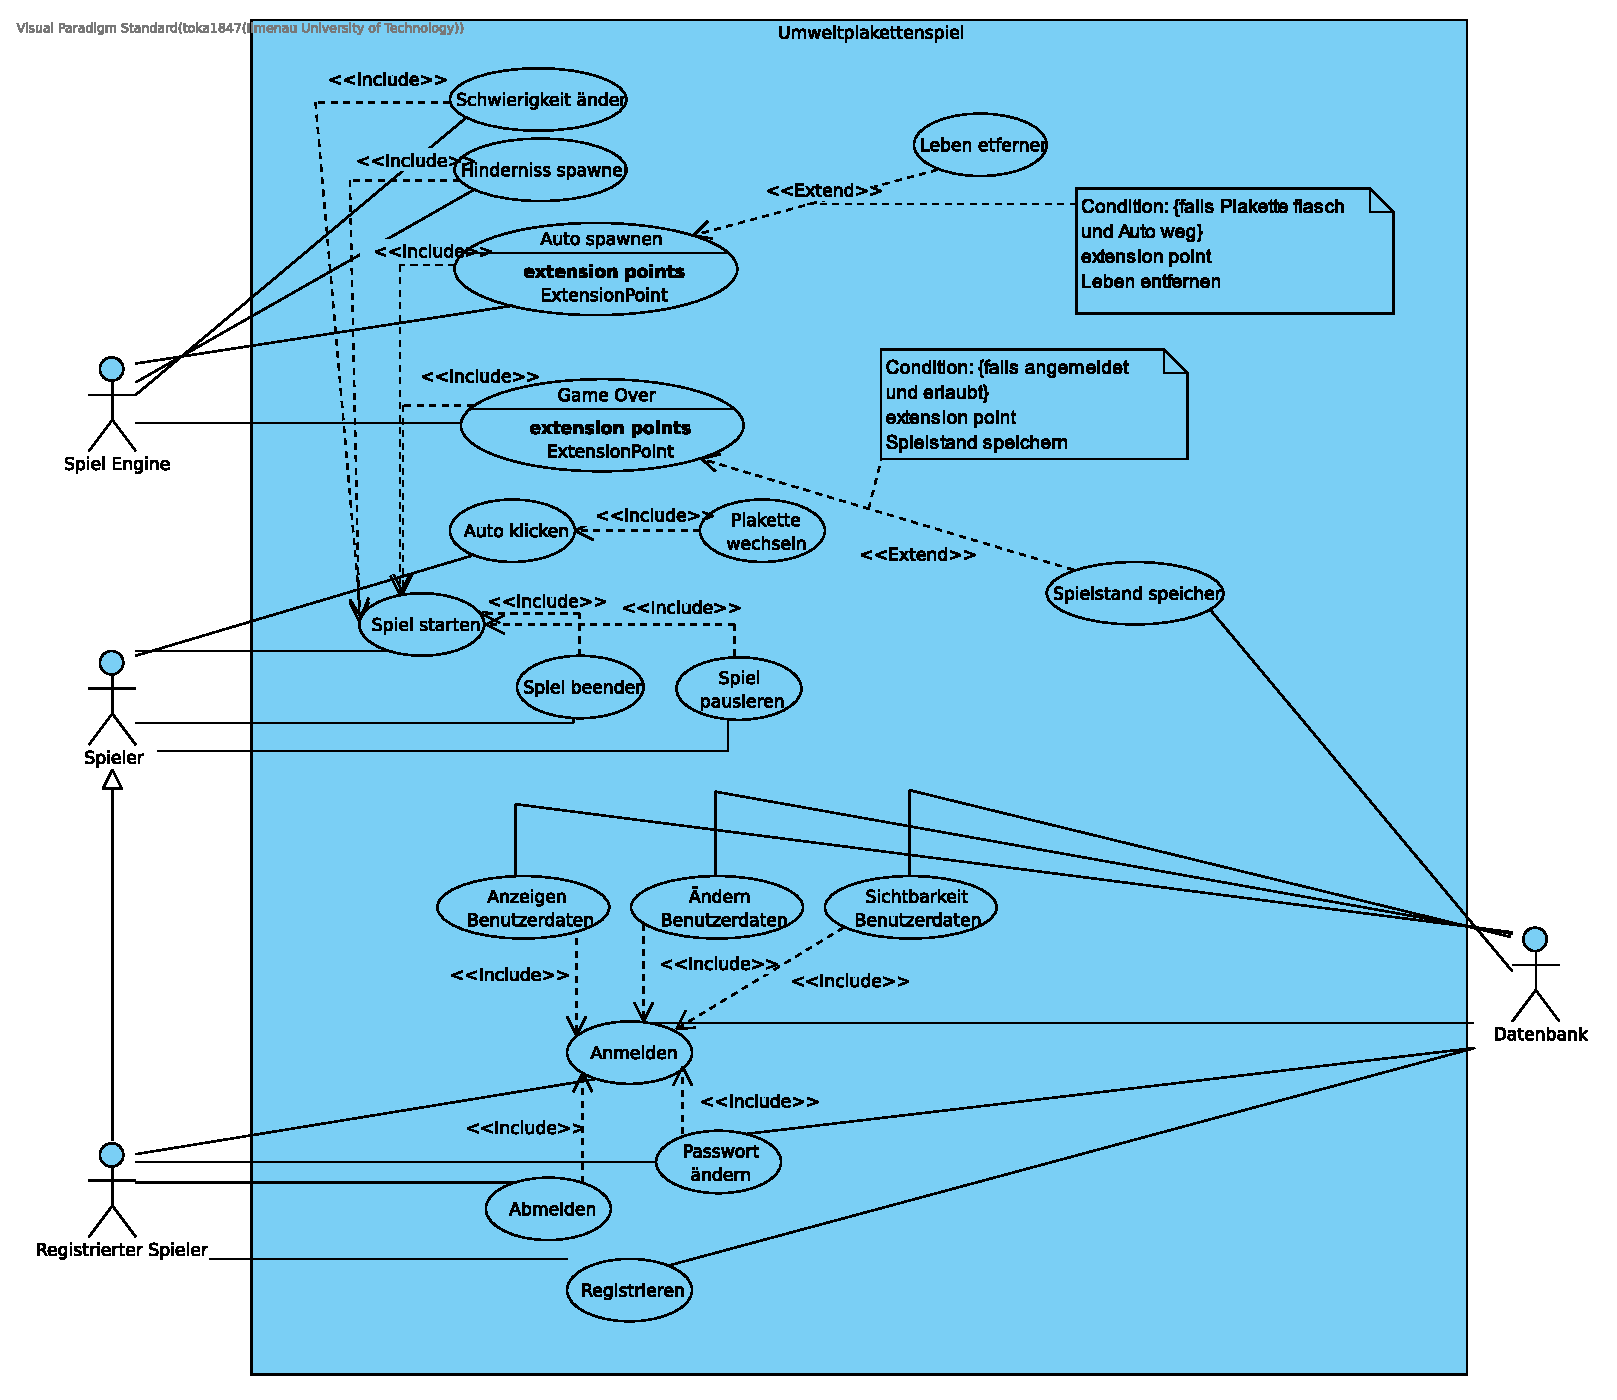
\includegraphics[width=\columnwidth]{res/seminar2-3.eps}
        \end{loesung}

%\end{fullpage}